\begin{table}[t!]
\scriptsize
\centering
\caption{Design delay, area and power numbers with and without {\sf Karna} for achieving a security ($\tau$) of 4.5.}
\label{tab:tvla}
\begin{tabular}{|p{1.2cm}|p{0.8cm}|p{0.8cm}|p{0.8cm}|p{0.8cm}|p{0.8cm}|p{0.8cm}|}
\hline
\multicolumn{1}{|l|}{\multirow{2}{*}}                              & \multicolumn{2}{c|}{\textbf{AES}}     & \multicolumn{2}{|c|}{\textbf{PRESENT} }  & \multicolumn{2}{|c|}{\textbf{Simon}}  \\ \cline{2-7} 
\multicolumn{1}{|l|}{}                                               & \textbf{\begin{tabular}[l]{@{}l@{}}Without \\ {\sf Karna}\end{tabular}} & \textbf{\begin{tabular}[l]{@{}l@{}}With\\ {\sf Karna}\end{tabular}} & \textbf{\begin{tabular}[l]{@{}l@{}}Without \\ {\sf Karna}\end{tabular}} & \textbf{\begin{tabular}[l]{@{}l@{}}With\\ {\sf Karna}\end{tabular}} & \textbf{\begin{tabular}[l]{@{}l@{}}Without \\ {\sf Karna}\end{tabular}} & \textbf{\begin{tabular}[l]{@{}l@{}}With\\ {\sf Karna}\end{tabular}}  \\ \hline
\textbf{Delay (ns)}                                                  & 0.5                                                                      & 0.5                                                                    & 0.3                                                                     & 0.3                                                                     & 1.12                                                                     & 1.12                                                                   \\ \hline
\textbf{\begin{tabular}[l]{@{}l@{}}Leakage\\Power($\mu$W)\end{tabular}}                                           & 492.4                                                                    & 236.65                                                                 & 5.62                                                                    & 0.418                                                                   & 3.70                                                                     & 0.16                                                                   \\ \hline
\textbf{\begin{tabular}[l]{@{}l@{}}Area\\  Utilization\end{tabular}} & 60\%                                                                     & 80\%                                                                   &          60\%                                                               &        81.8\%                                                                 &                             60\%                                             &        64.67\%                                                                \\ \hline 
\textbf{\#Gates}                                                     & 149943 & 149943                                                                                                                      & 1520 & 1520                                                                                                                         & 622  & 622                                                                                                                        \\ \hline
\textbf{Total Area (sq.microns)}  & 99651.67  &  99651.67 & 1596.9 & 1596.9 & 1240.3 & 1240.3 \\ \hline
\textbf{TVLA}                                                        & 8.22                                                                     & 3.7                                                                    & 12.28                                                                   & 4.06                                                                    & 20.799                                                                   & 4.48                                                                   \\ \hline
%\textbf{#Grids} &  & 100 &   & 1 &  & 1 \\ \hline

\end{tabular}
\vspace{-10pt}
\end{table}
\section{Implementation and Results}
\label{sec:experiment}
We use implementations of the AES\footnote{$https://opencores.org/projects/tiny\_aes$}, PRESENT\footnote{$https://opencores.org/projects/present$} and Simon\footnote{$https://opencores.org/projects/simon\_core$} ciphers to evaluate {\sf Karna} algorithm. For AES we set the grid size to $10\times 10$. PRESENT and Simon are very small designs, therefore a grid size of $1\times 1$ suffices.
The designs are synthesized using a 28nm standard cell library, which offers 3 $V_{dd}$ choices, 3 $V_t$ choices and 10 $size$ choices, thus a total of 90 configurations for every gate. We synthesize the designs for maximum performance using Synopsys design compiler version \texttt{M-2016.12-SP5-4} and use the Cadence innovus tool \texttt{v16.21-s078\_1} to place and route the design by setting the area utilization at 60\%. 

 The {\sf Karna} algorithm is implemented in C++. The implementation uses boost graph library version 1.58 to represent the netlist as a graph and the standard cell library to annotate the various power, delay and area information to each node. {\sf Karna} uses the power traces obtained from Synopsys PrimeTime \texttt{M-2017.06-SP2} to compute the TVLA. Each TVLA computation uses 4000 pairs of power traces for fixed and random test inputs. Based on the TVLA scores, the implementation identifies vulnerable gates and reconfigures them. It then invokes OpenTimer~\cite{Opentimer} to validate each reconfiguration.

 Table~\ref{tab:tvla} shows the properties of the synthesized netlist with and without {\sf Karna}. {\sf Karna} is able to achieve the desired level of security ($\tau=4.5$) in all three designs without any impact on delay, leakage power and the number of gates. While the total area of the chip remains the same, the area utilization increases by about 20\% for AES and PRESENT; and is negligible  for Simon. Figure~\ref{fig:aesfinal} shows the TVLA scores for various regions in the AES layout optimized for security using  {\sf Karna} after 100,000 power trace measurements.  Unlike the unoptimized AES layout (Figure~\ref{fig:aesopt}), we find no region having a TVLA score greater than 4.5.
 
The run time for the EDA flow with {\sf Karna} enabled is 3 days for AES and around 6 hours each for PRESENT and Simon on a 4-core Intel Xeon E5-1620 processor with 32 GB RAM. Almost 96\% of the time is taken up in collecting power traces for TVLA computation.
This is mainly because the TVLA computation in each iteration requires 8000 power traces to be simulated with different test vectors. This time  can be reduced by parallelizing trace collection.
%\vspace{-3pt}


%The EDA runtime depends considerably on the user specified security level $\tau$. A low value implies that the design is expected to meet strict security standards. This implies more regions in the netlist fail and consequently the module has to reconfigure a lot more gates. Figure~\ref{fig:tvla} shows that the number of grids that fail increases considerably as $\tau$ reduces. Thus for a small value of $\tau$, the algorithm will take longer to complete. 

%{\flushleft \bf Limitations of {\sf Karna}} The algorithm depends on the power traces to identify the vulnerable regions in each iteration. This trace collection drastically increases the runtime of the algorithm. For example, for the AES design, 73 minutes were spent in the EDA flow and 87 minutes were spent in the reconfiguration, however the trace collection took 3 days. In our future we explore methods to reduce this large time.



%Since, {\sf Karna} only reconfigures the gates in the netlist the overall gate count also remains constant. 


%The command allows for varying the granularity at which the dynamic power is calculated, and hence the TVLA analysis can be performed at any level the designer prefers. We set the security level to 4.5 and use a grid size of 100. 




% We use boost graph library. Each node in the graph has the following properties: node id, node type which could be a primary input/output or cell type, node slack, arrival time, output capacitance, number of gates driven by the particular node (fanouts), number of gates driving the particular node, $V_{dd}$, $V_t$, $size$, TVLA score. A node is marked unsafe if it belongs to a grid that has a high TVLA score and safe otherwise. A node is marked critical if it has timing violations or if it cannot be optimized further i.e, reconfiguring the node could lead to timing, slew or capacitance violations. The values of delay, leakage power and dynamic power are calculated based on the node type,$V_{dd}$, $V_t$ and $size$. %\cite{OpenTimer} has options for performing both full and incremental static timing analysis. We use the full STA option for our experiments. 

% The TVLA calculation was run on a 128-thread, 32-core dual socket AMD EPYC 7601 32-Core Processor. We sped up the trace collection by using the set\_host\_options command in primetime. 



% %describe the experimental setup.
% The AES netlist is synthesized using the 28nm netlist. Synopsys dc compiler version M-2016.12 was used to synthesize the netlist. The netlist has 150,000 gates The \textit{set\_max\_delay} option was used to ensure that the design is timing optimized. The target frequency was set at 0.5ns. The device is then placed and routed using innovus tool from cadence. 

% Around 40,000 traces are generated for the fixed and the varying inputs. The dynamic power calculation was done using synopsys primetime. The sampling was done using the \textit{read\_vcd} command in primetime. The command allows for varying the granularity at which the dynamic power is calculated, and hence the TVLA analysis can be performed at any level the designer wishes. The samples were collected using the experimental procedure described in \cite{}. 

%\section{Results}
% \todo{
% Include Present and Simon speck results. 
% }
\label{sec:results}

% We tested the {\sf Karna} algorithm on the following ciphers AES-128, Simon and PRESENT. Table~\ref{tab:tvla} shows the impact of {\sf Karna} algorithm on the design requirements such as Delay, Power and Area. It can be seen that overall 
% Figure~\ref{tvla} shows the variation in t-score with sample sizes. X-axis represents the number of samples while the Y-axis represents the t-score. It can be seen that the t-score crosses 4.5 even with 1000 samples. Figure~\ref{fig2} shows the t-score for each grid with 1000 samples. It can be seen that 21 grids fail out of the 100 grids. The gates belonging to these grids are considered for the optimization stage. Table ~\ref{tab:tvla} shows the variation in leakage power, delay, area of the netlist before and after optimization. 
% Please add the following required packages to your document preamble:
% \usepackage{graphicx}
% Please add the following required packages to your document preamble:
% \usepackage{multirow}






% Please add the following required packages to your document preamble:
% \usepackage{multirow}









% \begin{table*}[t!]
% \centering
% \caption{Table showing the delay, area and power numbers before and after optimization. While the area of the netlist increases, the total die area remains the same and hence the overall area of the manufactured device remains the constant.}
% \label{tab:tvla}

% \begin{tabular}{|c|c|c|}
% \hline
% \textbf{Parameter} & \textbf{\begin{tabular}[c]{@{}c@{}}Unoptimized \\ Netlist\end{tabular}} & \textbf{\begin{tabular}[c]{@{}c@{}}Optimized\\ Netlist\end{tabular}} \\ \hline
% \textbf{Delay(ns)} & 0.5 & 0.5 \\ \hline
% \textbf{Area(sq.microns)} & 59791 & 101502   \\ \hline
% \textbf{Static Power($\mu$W)} & 492.4  &  236.65  \\ \hline
% \textbf{TVLA score} & 8.22 & 3.7 \\ \hline
% %\textbf{Dynamic Power (mW)}
% \textbf{Total Number of Gates} &\multicolumn{2}{|c|}{149943} \\ \hline
% \end{tabular}%
% \end{table*}
%\subsection{Runtime Optimizations of {\sf Karna}}
% As mentioned in Section~\ref{sec:proposed}, the number of STA calls can have an impact on the overall runtime of the algorithm. In order to reduce the number of STA calls, we use an adaptive gate replacement policy used in~\cite{MLtimer} in order to speed up the {\sf Karna} module. Figure~\ref{fig:runtime} shows the speedup achieved by employing this gate replacement policy. It can be seen that adaptive window sizing policy is $\approx5\times$ faster than the greedy replacement policy. This is because the order in which the gates get replaced remains fairly constant for most of the iterations, an observation which we leverage to converge to an optimal solution faster.

\begin{figure}[t!]
\centering
  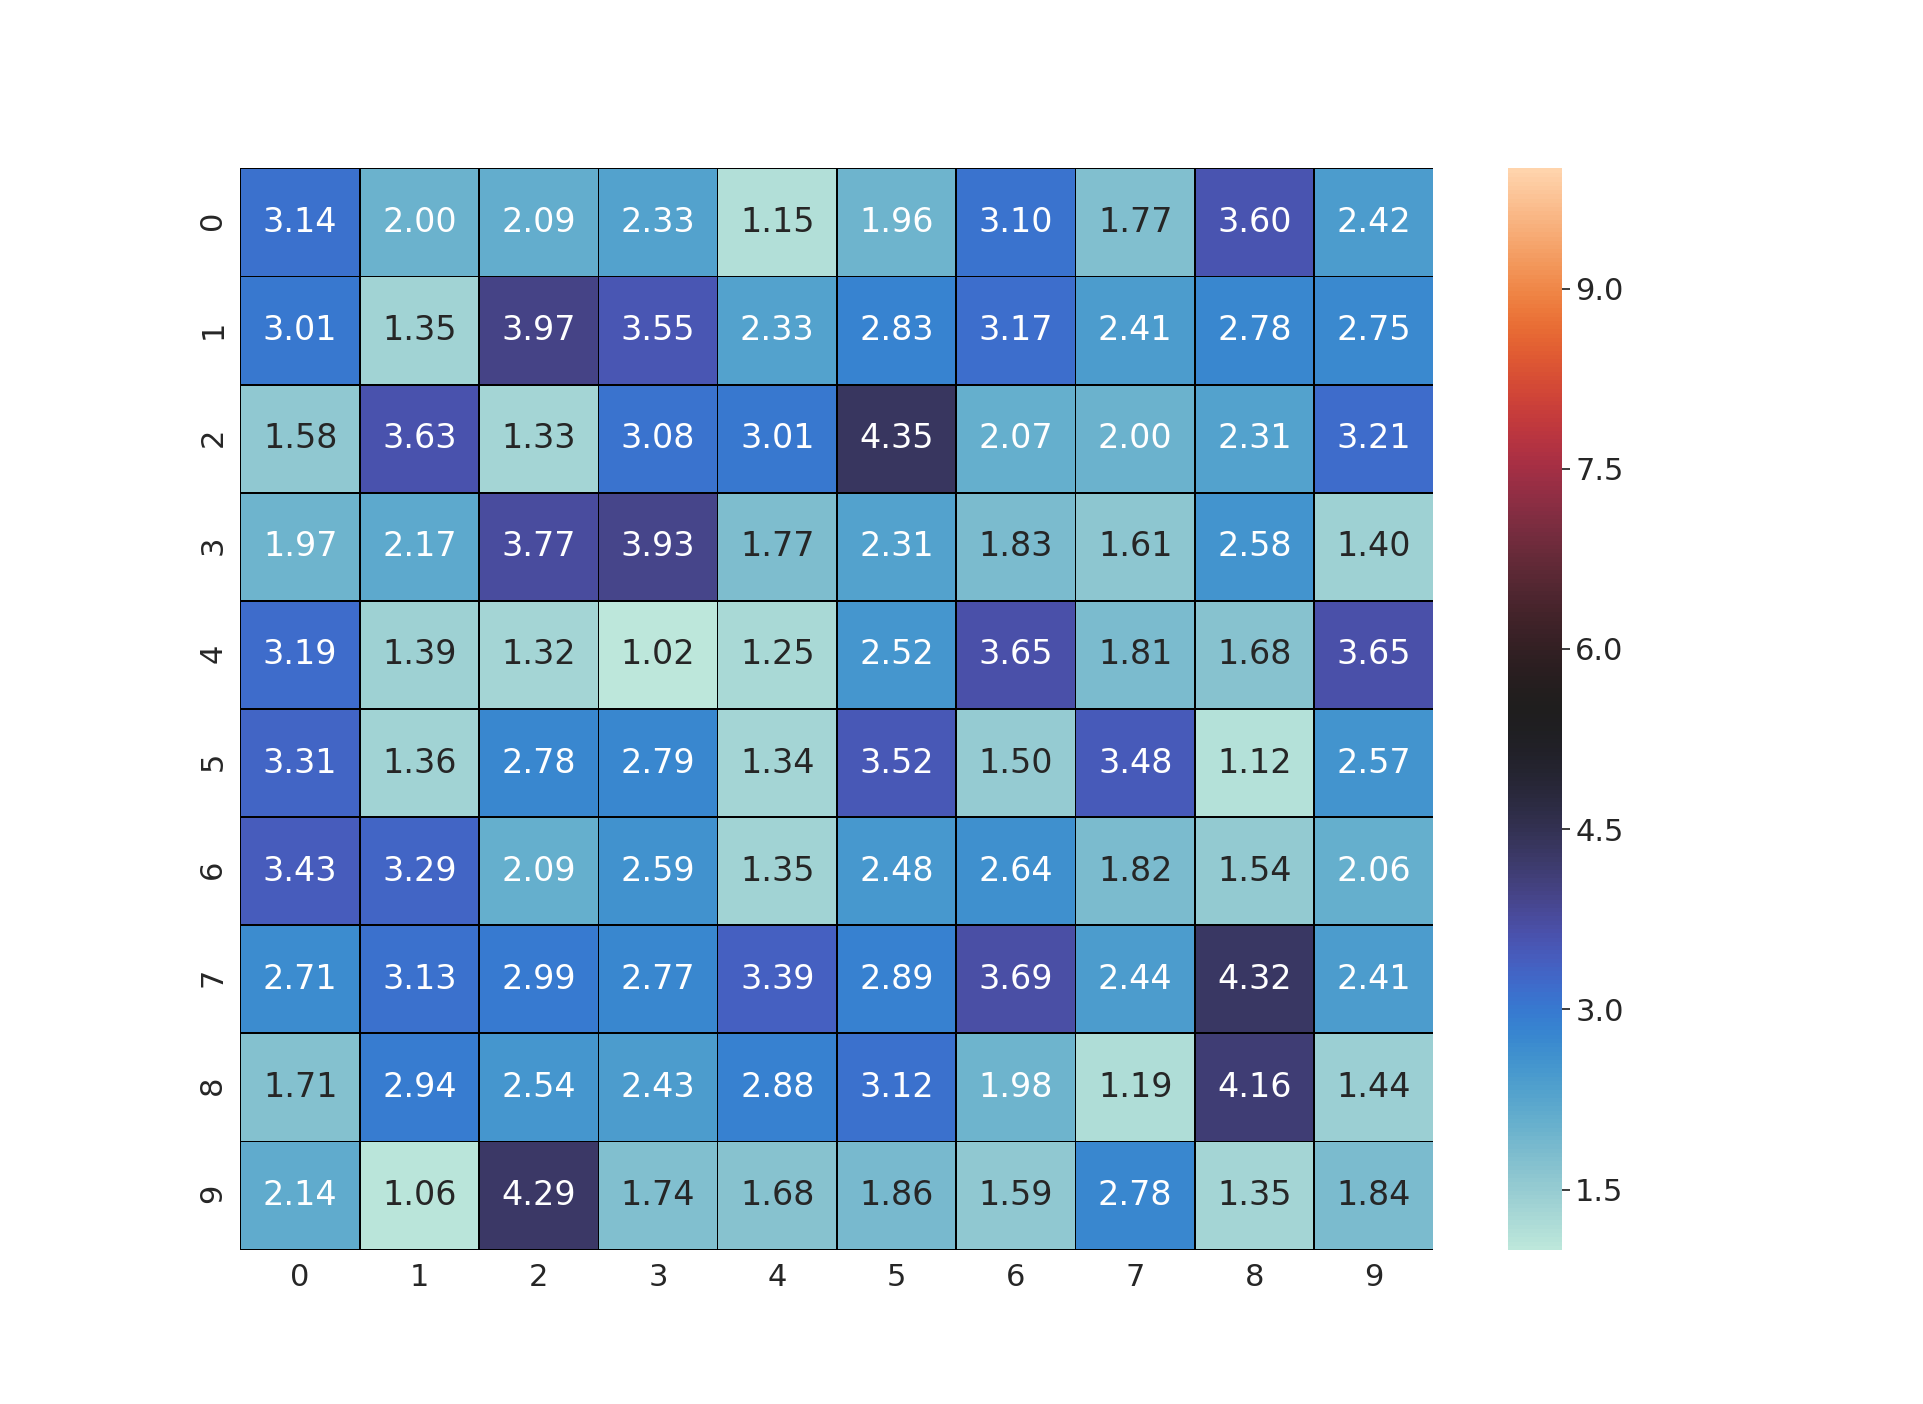
\includegraphics[scale=0.20]{Chapter4/fig/aes_final.png}  
\caption{The TVLA profile of the AES-128 design, with the design divided into a $10\times 10$ grid after {\sf Karna} optimization. }
\label{fig:aesfinal}
\vspace{-10pt}
\end{figure}


% \begin{figure}[t!]
% \centering
% 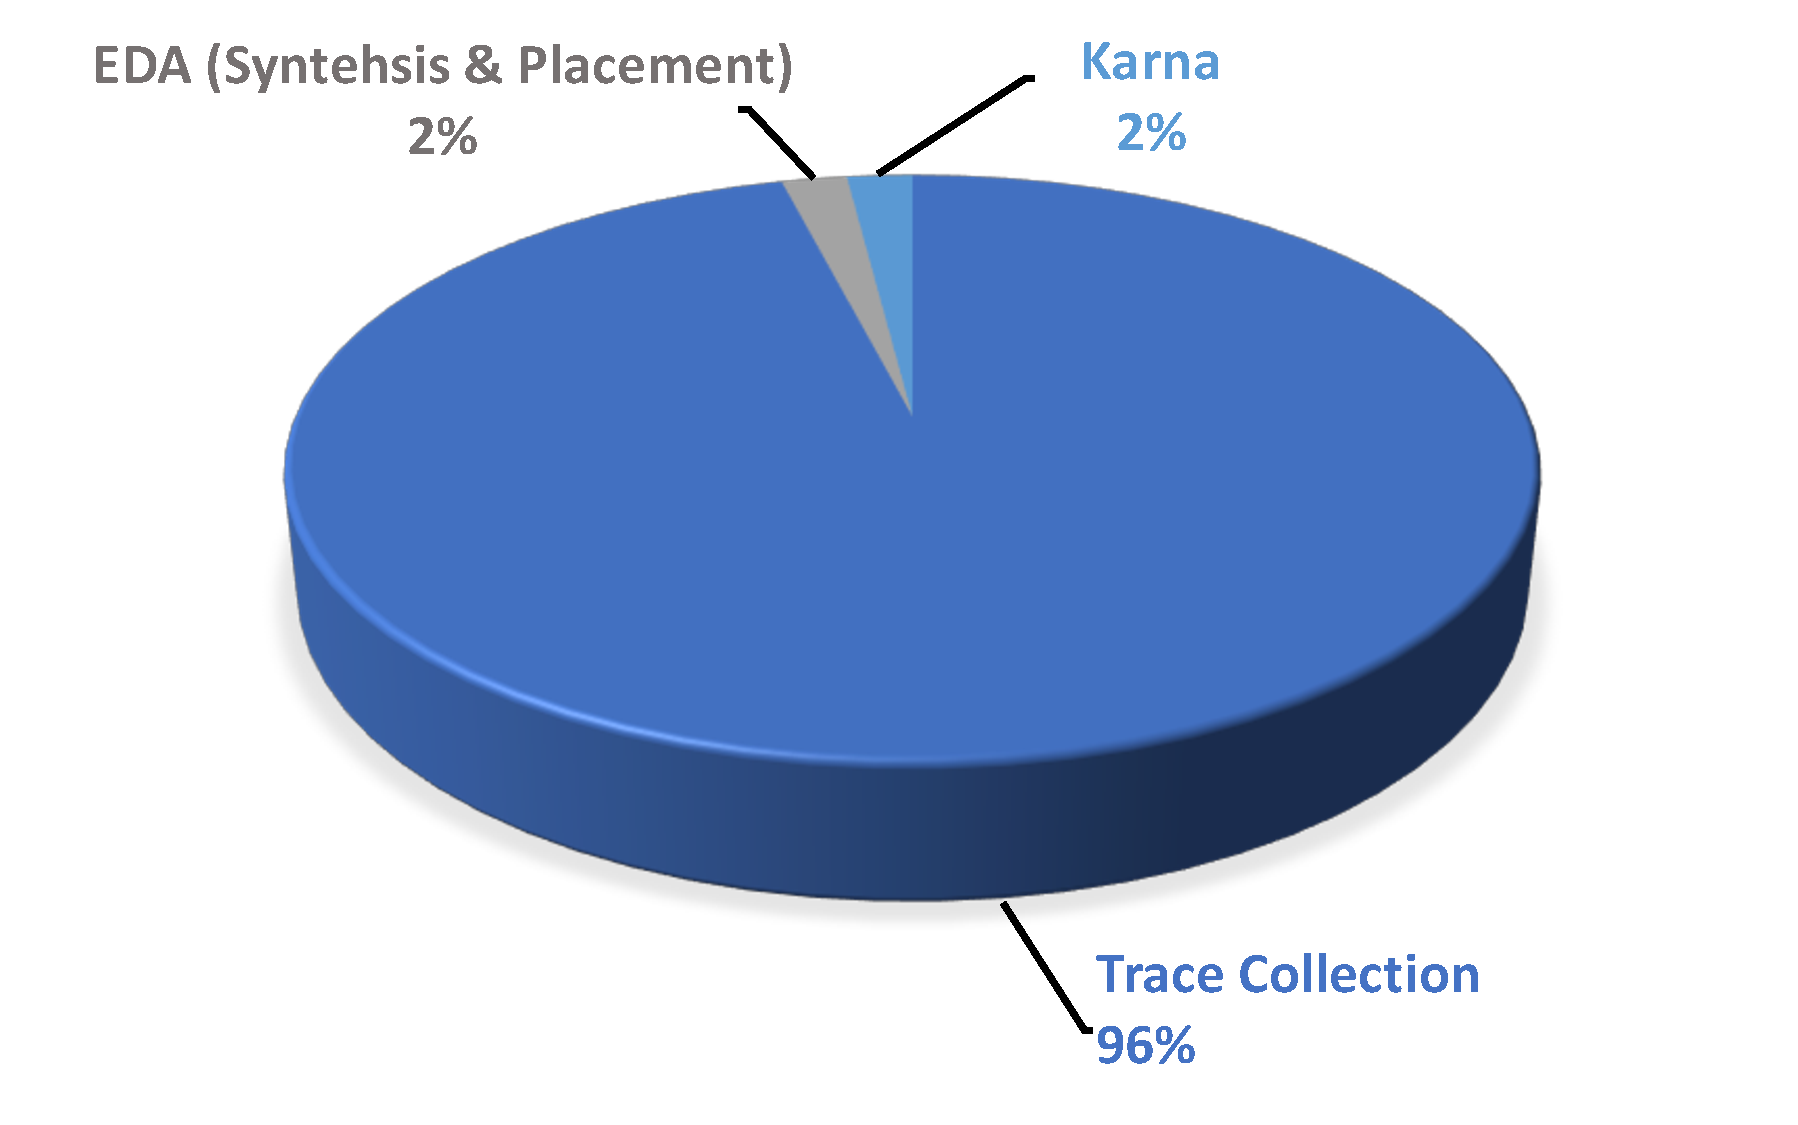
\includegraphics[scale=0.20]{fig/aespie.pdf}
% \caption{Distribution of run time for the AES design}
% \label{fig:aespie}
% \vspace{-15pt}
% \end{figure}


% \begin{figure}[ht!]
% \centering
% 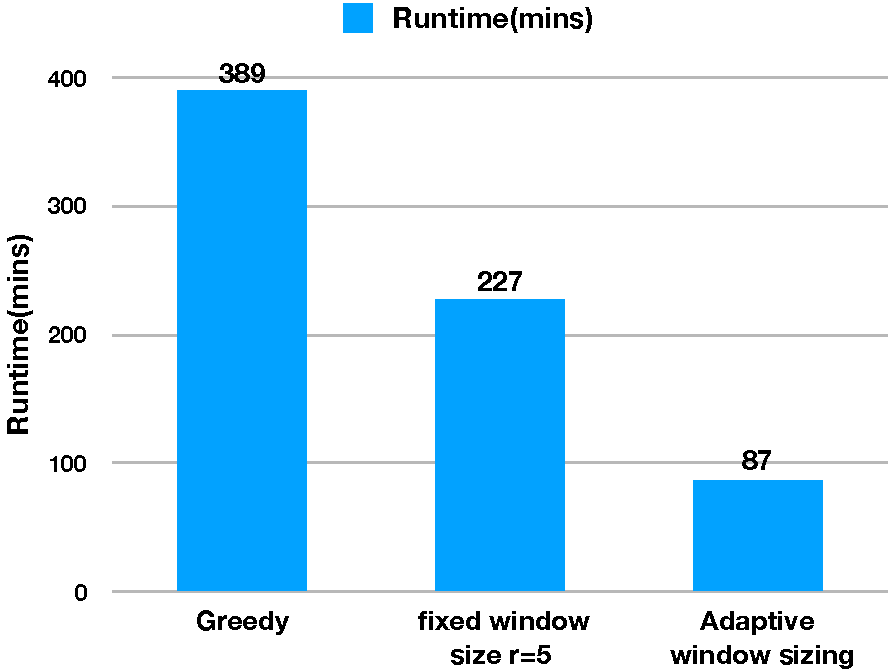
\includegraphics[scale=0.45]{fig/runtime.pdf}
% \caption{Figure showing the variation of runtime with different optimization.}
% \label{fig:tvla}
% \end{figure}





% \section{Discussion}
% \todo[inline]{Convergence of the Karna algorithm with CMOS technology}
% \todo[inline]{The effect of grid size}
% In this section, we discuss the various factors that could affect the convergence of {\sf Karna} algorithm to an optimal solution. 

% \subsection{Number of grids $N_{grids}$} 
 

% \subsection{Standard cell library Technology scaling} 
% The number of $V_{dd}$, $V_{t}$ amd size options influence the overall solution quality and runtime. If the number of options are limited it restricts the ability of the {\sf Karna} algorithm to converge to an optimal solution. However, limiting the number of options will speed up the algoritm as for every gate the number of options that need to be considered are lesser. For example, limiting the number of 
% \subsection{Initial TVLA score}
%It should be noted that the
